\documentclass[12pt]{report}

\usepackage[a4paper, margin=1in]{geometry}

\usepackage[english]{babel}
\usepackage{amsmath} % Add this in the preamble
\usepackage{amssymb}
\usepackage{enumitem}
\usepackage{tikz}


\begin{document}
	
	\chapter{Introduction}
	
	\chapter{Toric Code}
	\section{Model}
	
	
	\begin{minipage}{1\textwidth}
		
		The toric code model is defined on a square lattice with periodic boundary conditions in both directions; these latter characteristics in topology are typical of what is known as a torus topology or simply a Torus, from which the name of the model.\newline
		
		A square lattice $L$ is a particular lattice defined in a two dimensional Euclidian space. It is denoted as $\mathbb{Z}^{2}$, such that each lattice point is identified with a tuple of integers. Though, the above mentioned boundary conditions also specify that for any point $(i, j)$ in the lattice, the neighboring points are going to be the following: $(i+1 \ mod \ L, j)$, $(i-1 \ mod \ L, j)$, $(i, j+1 \ mod \ L)$, and $(i, j-1 \ mod \ L)$.  \newline
		
		In our case, we are also going to consider a dual lattice, which will be denoted as $L'$ and that will be positioned in the following way.\newline
		
		\begin{center}
		
		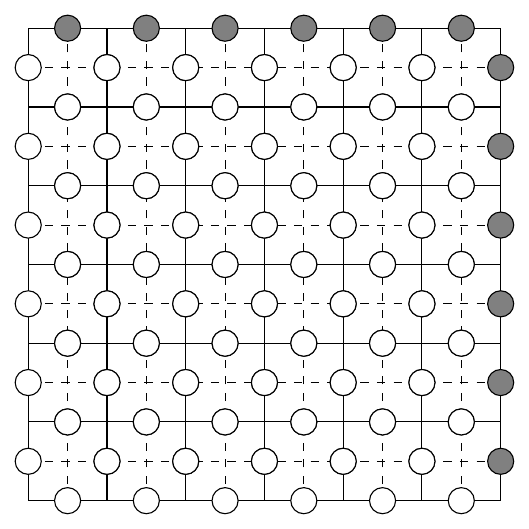
\begin{tikzpicture}
			% Draw dashed lines
			\foreach \i in {-3,-2.5,...,3}
			{
				\draw[dashed] (\i,-3) -- (\i,3);
			}
			\foreach \j in {-3,-2.5,...,3}
			{
				\draw[dashed] (-3,\j) -- (3,\j);
			}
			
			% Draw solid grid and nodes with circles in the middle of each side
			\draw[step=1cm] (-3,-3) grid (3,3);
			\foreach \i in {-2.5,...,2.5}
			{
				\foreach \j in {-2.5,...,2.5}
				{
					\begin{scope}[transform canvas={xshift=\i cm,yshift=\j cm}]
						\node[right,xshift=0.2cm,yshift=0.4cm] {};
						% Convert \j and \i to integers
						\pgfmathtruncatemacro{\intj}{\j}
						\pgfmathtruncatemacro{\inti}{\i}
						
						% Draw circles at the midpoints of each side
						\ifnum\intj=2
						\draw node[draw,circle,fill=gray] at (0,0.5) {};
						\else
						\draw node[draw,circle,fill=white] at (0,0.5) {};
						\fi
						
						\ifnum\inti=2
						\draw node[draw,circle,fill=gray] at (0.5,0) {};
						\else
						\draw node[draw,circle,fill=white] at (0.5,0) {};
						\fi
						
						\draw node[draw,circle,fill=white] at (0,-0.5) {};
						\draw node[draw,circle,fill=white] at (-0.5,0) {};
					\end{scope}
				}
			}
		\end{tikzpicture}
		
	    \end{center}
	    
	    The continuous line represents the main lattice $L$, while the dashed line represents its dual $L'$.\newline 
		On each edge is located a spin-$\frac{1}{2}$ particle, i.e. a Fermion (or Electron), represented in the image above with an empty circle.
		For each cell of $L$ we are going to consider two spins, therefore the total number of spins will correspond to $2N$, where $N$ represents the total number of cells in $L$ and the dimension of the lattice. \newline
		Since all of these spins exhibit the same characteristics they are identcial particles, which will be useful to know to study further properties of the model.
	
	\end{minipage}
	
	
	\begin{minipage}{1\textwidth}
		
		The above mentioned cells in the Toric model are called "plaquettes", while the lattice points are called "verteces".
		Then, in order to complete the description of the model we define the following operators as the main actors of the model:\newline
		
		\textbf{Definition 2.1.1.} (Vertex and Plaquette operators) Given a vertex $v$ and a plaquette $p$, we can define the following vertex and plaquette operators as tensor products over Pauli operators acting on individual spins indicated by the indices $j \in star(v)$ and $j \in bdy(p)$  \newline 
		
		\begin{center}
			$ Av = \prod_{j \in star(v)} Z_j $ \newline
			
			$ Bp = \prod_{j \in bdy(v)} X_j $.\newline
		\end{center}
		
		The $Av$ operator is going to be shaded in blu, while the $Bp$ operator will be coloured in red, as exemplified in the picture below. \newline
		
		\begin{center}
		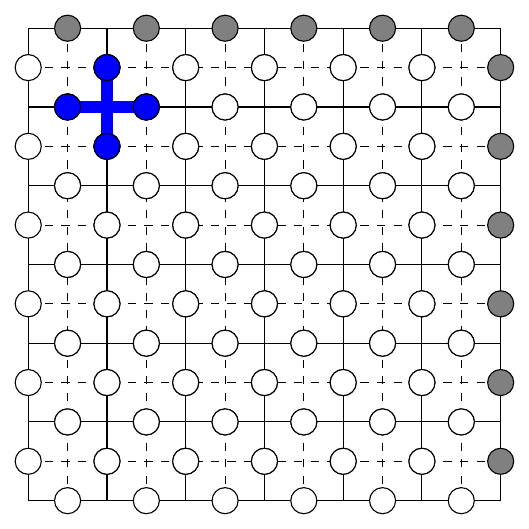
\begin{tikzpicture}
				% Draw dashed lines
				\foreach \i in {-3,-2.5,...,3}
				{
					\draw[dashed] (\i,-3) -- (\i,3);
				}
				\foreach \j in {-3,-2.5,...,3}
				{
					\draw[dashed] (-3,\j) -- (3,\j);
				}
				
				
				
				% Draw solid grid and nodes with circles in the middle of each side
				\draw[step=1cm] (-3,-3) grid (3,3);
				\foreach \i in {-2.5,...,2.5}
				{
					\foreach \j in {-2.5,...,2.5}
					{
						
						
						\begin{scope}[transform canvas={xshift=\i cm,yshift=\j cm}]
							\node[right,xshift=0.2cm,yshift=0.4cm] {};
							% Convert \j and \i to integers
							\pgfmathtruncatemacro{\intj}{\j}
							\pgfmathtruncatemacro{\inti}{\i}
							
							% Draw circles at the midpoints of each side
							\ifnum\intj=2
							\draw node[draw,circle,fill=gray] at (0,0.5) {};
							\else
							\draw node[draw,circle,fill=white] at (0,0.5) {};
							\fi
							
							\ifnum\inti=2
							\draw node[draw,circle,fill=gray] at (0.5,0) {};
							\else
							\draw node[draw,circle,fill=white] at (0.5,0) {};
							\fi
							
							\draw node[draw,circle,fill=white] at (0,-0.5) {};
							\draw node[draw,circle,fill=white] at (-0.5,0) {};
						\end{scope}
					}
				}
				
				\foreach \i in {-2,...,-2}
				{
					
					\draw[blue, line width=1.5mm] (\i,1.5) -- (\i,2.5);
					\node[draw, circle, fill=blue] at (\i,1.5) {};
					\node[draw, circle, fill=blue] at (\i,2.5) {};
					
				}
				\foreach \j in {2,...,2}
				{
					
					\draw[blue, line width=1.5mm] (-2.5, \j) -- (-1.5, \j);
					\draw node[draw,circle,fill=blue] at (-2.5,\j) {};
					\draw node[draw,circle,fill=blue] at (-1.5,\j) {};
					
				}
				
		\end{tikzpicture}
		\end{center}
		
		Given definition 2.1.1., we can now write the Hamiltonian of the whole system as follows:\newline
		
		\textbf{Definition 2.1.2.} (Toric Code Hamiltonian) Given the application sites v and p of  respectively, vertex and plaquette operators, and given spin-$\frac{1}{2}$ particles located on each edge of the torus, we can define the following Hamiltonian for the system:\newline
		
		\begin{center}
			
			$H = -\sum_{v} 
			Av - \sum_{p} Bp $.\newline
			
		\end{center}
		
		Each one of the $Av$ and $Bp$ operators that appear in the Hamiltonian share some important properties, which are going to be covered in the following definitions and will later be used to further characterize the action of the operators. \newline
		
		
		Firstly, notice that $Av$ and $Bp$ operators are Hermitian and square to the identity. \newline
		
	\end{minipage}  
	
	
	\begin{minipage}{1\textwidth}	
		
		
		\textbf{Definition 2.1.3.} (Hermitian operator) Let $V$ be  a finite dimensional vector space over $\mathbb{C}$, with a fixed positive definite hermitian product defined as $<v,w>$ for $v,w \in V$. Let $A$: $V \rightarrow V$ be a linear map. An operator is called Hermitian (or self-adjoint) if $A^H=A$. This means that for all $u,v \in V$ we have\newline
		
		\begin{center}
			$<Av,w> = <v,Aw>$.
		\end{center}
		
		In particular, it is important for the following applications to specify that a square matrix $A$ of complex numbers is called hermitian if $(A^*)^T = A$, i.e. if the conjugate-transpose of $A$ is equal to $A$ itself. Note also that for real matrices it is sufficient to compute only the transpose of the matrix to verify hermiticity. \newline
		
		Then, the involutory property comes from the unitarity of the matrices representing the vertex and plaquette operators, i.e. $X$ and $Z$ Pauli matrices, which are real matrices. \newline
		
		\textbf{Definition 2.1.4.} (Unitary operator) Let $V$ be  a finite dimensional vector space over $\mathbb{C}$, with a positive definite hermitian product. Let $A$: $V \rightarrow V$ be a linear map. We define A to be complex unitary if \newline
		
		\begin{center}
			$<Av,Aw> = <v,w>$.
		\end{center}
		
		for all $v,w \in V$. We can define a complex matrix $A$ to be unitary if $ (A^*)^T=A^{-1}$. We note that it is possible to define an operator to be real unitary, with the only difference that $(A)^T = A^{-1}$. Then, we can also define that a real matrix is unitary if $(A)^T = A^{-1}$ or, equivalently, if $(A)^T A=I$.\newline
		
		Given the considerations made in Definition 2.1.3. and 2.1.4. for ral matrices, we can easily prove the first following proposition: \newline
		
		textbf{Proposition 2.1.1.} (Hermiticity and involutory property of $Av$ and $Bp$ operators)
		$Av$ and $Bp$ operators are Hermitian and satisfy the involutory property.\newline
		
		\textit{Proof}\newline
		
		We know that the operator $ Av = \prod_{j \in star(v)} Z_j $ and that $ Bp = \prod_{j \in bdy(v)} X_j $ .\newline
		
		Firstly, recall the form of the $\sigma_x$ and $\sigma_z$ matrices representing the Pauli gates $X$ and $Z$:
		
		
		
		\[
		\text{Z = $\sigma_z$} =
		\begin{bmatrix}
			1 & 0 \\
			0 & -1
		\end{bmatrix}
		\]
		
		
		\[
		\text{X = $\sigma_x$} =
		\begin{bmatrix}
			0 & 1 \\
			1 & 0
		\end{bmatrix}
		\]
		
		
	\end{minipage}  
	
	
	\begin{minipage}{1 \textwidth}
			Prove that they are Hermitian:\newline
		
		\[
		\text{$( \sigma_z )^{H}$} = 
		\begin{bmatrix}
			1 & 0 \\
			0 & -1
		\end{bmatrix} ^H =
		\begin{bmatrix}
			1 & 0 \\
			0 & -1
		\end{bmatrix}^T =
		\begin{bmatrix}
			1 & 0 \\
			0 & -1
		\end{bmatrix}
		= \text{$ \sigma_z $}
		\]
		
		
		\[
		\text{$( \sigma_x )^{H}$} = 
		\begin{bmatrix}
			0 & 1 \\
			1 & 0
		\end{bmatrix} ^H =
		\begin{bmatrix}
			0 & 1 \\
			1 & 0
		\end{bmatrix}^T =
		\begin{bmatrix}
			0 & 1 \\
			1 & 0
		\end{bmatrix}
		= \text{$ \sigma_x $}
		\]\newline
		
		Note that Pauli matrices are real matrices, i.e. $A^H=A^T$.
		Then, knowing that $[\sigma_i,\sigma_j]=0 \ for \ i=j$ we can write		\newline
		
		\begin{center}
			$(Av)^{H} = (\sigma_{x_1} \sigma_{x_2} \sigma_{x_3} \sigma_{x_4})^{H} = \sigma_{x_1}^H \sigma_{x_2}^H \sigma_{x_3}^H \sigma_{x_4}^H = \sigma_{x_1} \sigma_{x_2} \sigma_{x_3} \sigma_{x_4} = Av$ \newline
			
			$(Bp)^{H} = (\sigma_{z_1} \sigma_{z_2} \sigma_{z_3} \sigma_{z_4})^{H} = \sigma_{z_1}^H \sigma_{z_2}^H \sigma_{z_3}^H \sigma_{z_4}^H = \sigma_{z_1} \sigma_{z_2} \sigma_{z_3} \sigma_{z_4} = Bp$\newline
		\end{center}
		
		Prove the involutory propertyy:\newline
		
		\[
		\text{$( \sigma_z )^{2}$} = 
		\begin{bmatrix}
			1 & 0 \\
			0 & -1
		\end{bmatrix} *
		\begin{bmatrix}
			1 & 0 \\
			0 & -1
		\end{bmatrix} =
		\begin{bmatrix}
			1 & 0 \\
			0 & 1
		\end{bmatrix}
		= \text{$I$}
		\]
		
		
		\[
		\text{$( \sigma_x )^{2}$} = 
		\begin{bmatrix}
			0 & 1 \\
			1 & 0
		\end{bmatrix} *
		\begin{bmatrix}
			0 & 1 \\
			1 & 0
		\end{bmatrix} =
		\begin{bmatrix}
			1 & 0 \\
			0 & 1
		\end{bmatrix}
		= \text{$I$}
		\]\newline
		
		
		Then, again we can write\newline
		
		\begin{center}
			$(Av)^{2} = (\sigma_{x_1} \sigma_{x_2} \sigma_{x_3} \sigma_{x_4})^{2} = \sigma_{x_1}^2 \sigma_{x_2}^2 \sigma_{x_3}^2 \sigma_{x_4}^2 = I$ \newline
			
			$(Bp)^{2} = (\sigma_{z_1} \sigma_{z_2} \sigma_{z_3} \sigma_{z_4})^{2} = \sigma_{z_1}^2 \sigma_{z_2}^2 \sigma_{z_3}^2 \sigma_{z_4}^2 = I$\newline
		\end{center}
		
		\hfill $\square$\newline
	\end{minipage}
	
	
	\begin{minipage}{1\textwidth}
		
		
		Given Proposition 2.1.1., we can know further characterize the opeartors in terms of their eigenvalues and define their spectrum.	\newline
		
		\textbf{Proposition 2.1.2.} (Eigenvalues of $Av$ and $Bp$ operators) Given $Av$ and $Bp$ operators Hermitian and satisfying the involutory property, their eigenvalues are $\pm 1$.
		\newline
		
		\textit{Proof}\newline
		
		Given the Hermiticity and involutory proof in 2.1.1, we prove that Hermitian operators (and therefore our vertex and plaquette operators) have real eigenvalues: \newline
		
		Write the expression for the eigenvalues $Av |\xi> = \lambda |\xi>$ and take as hypothesis that $|\xi> \neq 0$. Then, by means of the scalar product\newline
		
		\begin{center}
			$<\xi|Av|\xi> = \lambda <\xi |\xi>$\newline
			
			$\lambda = \frac {<\xi|Av|\xi>}{<\xi |\xi>}$ = $\frac {<\xi|Av|\xi>}{||\xi||^2}$ = $\frac {<\xi|Av^H|\xi>}{||\xi||^2}$ = $\frac {<\xi|Av|\xi>^*}{||\xi||^2}$ = $\lambda^*$\newline
		\end{center}
		
		Note that we applied antidistributivity: \newline
		
		\begin{center}
			$(<\xi|Av^H|\xi>)^H$ = $|\xi>^H (Av^H)^H <\xi|^H$ = $<\xi|Av|\xi>^*$. \newline
		\end{center}
		
		Using hermiticity with the fact that $(Av)^2=I$ we can derive the unitarity of $Av$ and state that $Av Av^H = Av^H Av = (Av)^2 = I$, i.e. for a unitary operator $U$ we have $U^H=U^{-1}$. \newline
		
		One property of unitary operators states that their eigenvalues have modulus equal to one:\newline 
		
		
		By taking as hypothesis $|\xi> \neq 0$, we write the expression $U |\xi> = \lambda |\xi>$ and its self-adjoint $<\xi| U^H = \lambda^* <\xi|$. Then, knowing that $U^H=U^{-1}$, by means of the scalar product we obtain \newline
		
		\begin{center}
			$<\xi|U U^H|\xi> = \lambda \lambda^* <\xi |\xi>$\newline
			
			$<\xi|I|\xi> = \lambda \lambda^* <\xi |\xi>$\newline
			
			$<\xi|\xi> = \lambda \lambda^* <\xi |\xi>$\newline
		\end{center}
		
		Finally, since we already know that Hermitian operators have real eigenvalues we can write $|\lambda|^2 = 1$.\newline
		
		Putting together the fact that $Av$ has real eigenvalues with unitarity we obtain that the only two remaining possibilities for the eigenvalues of $Av$ are $\pm 1$. \newline
		
		
		
	\end{minipage}
	
	\begin{minipage}{1\textwidth}
		
		The same reasoning can be carried out for the $Bp$ operator.
		
		\hfill $\square$ \newline
		
		Given the result of proposition 2.1.2., the spectrum of the operators is easy to find:	\newline
		
		\textbf{Proposition 2.1.3.} (Spectrum of $Av$ and $Bp$ operators) The spectrum of $Av$ and $Bp$ operators is $ \sigma \ = \ \{-1,+1\}$. \newline
		
		We now analyze the relationship between vertex and plaquette operators. Such relationship is characterized by two fundamental mathematical concepts called "commutation" and "anticommutation". These relations serve as an important result in understanding the stability and fault-tolerance of the toric code.	\newline
		
		\textbf{Proposition 2.1.4.} (Commutation of $Av$ and $Bp$ operators) The operator Av commutes with the operator Bp for an even number of edges.
		\newline
		
		\textbf{Proposition 2.1.5.} (Anticommutation of $Av$ and $Bp$ operators) The operator $Av$ anticommutes with the operator $Bp$ for an odd number of edges.
		\newline
		
		\textit{Proof}\newline 
		%Av commutes with itself.\newline
		%Bp commutes with itself.\newline
		%Av commutes with Bp for an even number of edges.\newline
		
		Fix the origin of the coordinate system in the bottom left corner of the lattice as indicated in the picture below:\newline
		
		%picture
		
		then, we can define the two vectors representing the site of application of the vertex and plaquette operator, respectively over the lattice L and dual lattice L'
		
		\begin{center}
			$\vec{v}$= $n\hat{e_1} + m\hat{e_2}$, where $n,m \in \mathbb{Z}$ \newline
			
			$\vec{p}$= $(n + \frac{1}{2}) \hat{e_1} + (m + \frac{1}{2}) \hat{e_2}$, where $n,m \in \mathbb{Z}$\newline
		\end{center}
		
		Rewrite the operators as follows:\newline
		
		\begin{center}
			
			$A_{\vec{v}} = \sigma^z_{\vec{v}+\frac{1}{2}\hat{e_1}} \sigma^z_{\vec{v}+\frac{1}{2}\hat{e_2}} \sigma^z_{\vec{v}-\frac{1}{2}\hat{e_1}} \sigma^z_{\vec{v}-\frac{1}{2}\hat{e_2}}$ \newline
			
			$B_{\vec{p}} = \sigma^x_{\vec{p}+\frac{1}{2}\hat{e_1}} \sigma^x_{\vec{p}+\frac{1}{2}\hat{e_2}} \sigma^x_{\vec{p}-\frac{1}{2}\hat{e_1}} \sigma^x_{\vec{p}-\frac{1}{2}\hat{e_2}}$\newline
			
		\end{center}
		
		In order to simplify the calculations we rewrite $Bp$ on the lattice L by rewriting the indeces in terms of vector $\vec{v}$
		
		\begin{center}
			$(n\hat{e_1} + m\hat{e_2}) + \frac{1}{2}\hat{e_2}= n\hat{e_1} + (m+\frac{1}{2}\hat{e_2})$\newline
			
			$(n\hat{e_1} + m\hat{e_2}) + \frac{1}{2}\hat{e_1}= (n+ \frac{1}{2})\hat{e_1} + m\hat{e_2}$\newline
			
			$(n\hat{e_1} + m\hat{e_2}) + \frac{1}{2}\hat{e_1}+\hat{e_2}= (n+ \frac{1}{2})\hat{e_1} + (m + 1)\hat{e_2}$\newline
			
			$(n\hat{e_1} + m\hat{e_2}) + \frac{1}{2}\hat{e_2}+\hat{e_1}= (n+ 1)\hat{e_1} + (m + \frac{1}{2})\hat{e_2}$\newline
		\end{center}
		
		
		
		
	\end{minipage}
	
	\begin{minipage}{1\textwidth}
		
		Then the $B_{\vec{p}}$ operator becomes:
		
		\begin{center}
			
			$B_{\vec{v}} = \sigma^x_{n\hat{e_1} + (m+\frac{1}{2}\hat{e_2})} \sigma^x_{(n+ \frac{1}{2})\hat{e_1} + m\hat{e_2}} \sigma^x_{(n+ \frac{1}{2})\hat{e_1} + (m + 1)\hat{e_2}} \sigma^x_{(n+ 1)\hat{e_1} + (m + \frac{1}{2})\hat{e_2}}$\newline
			
		\end{center}
		
		
		
		and the Hamiltonian can be written by grouping the indices:\newline
		
		\begin{center}
			
			$H = - \sum_{m,n \in \mathbb{Z}} \{ 
			\sigma^z_{(n+\frac{1}{2})\hat{e_1} + m\hat{e_2}} \sigma^z_{n\hat{e_1}+(m+\frac{1}{2})\hat{e_2}} \sigma^z_{(n-\frac{1}{2})\hat{e_1} + m\hat{e_2}} \sigma^z_{n\hat{e_1}+(m-\frac{1}{2})\hat{e_2}} +
			\sigma^x_{n\hat{e_1} + (m+\frac{1}{2}\hat{e_2})} \sigma^x_{(n+ \frac{1}{2})\hat{e_1} + m\hat{e_2}} \sigma^x_{(n+ \frac{1}{2})\hat{e_1} + (m + 1)\hat{e_2}} \sigma^x_{(n+ 1)\hat{e_1} + (m + \frac{1}{2})\hat{e_2}} \} $
			
		\end{center}
		
		Now calcuate the commutator $[A_{\vec{v}},B_{\vec{v}}] = A_{\vec{v}}B_{\vec{v}} - B_{\vec{v}}A_{\vec{v}}$ by focusiing on the first term:\newline
		
		\begin{center}
			
			$ A_{\vec{v}}B_{\vec{v}} =
			\sigma^z_{(n+\frac{1}{2})\hat{e_1} + m\hat{e_2}} \sigma^z_{n\hat{e_1}+(m+\frac{1}{2})\hat{e_2}} \sigma^z_{(n-\frac{1}{2})\hat{e_1} + m\hat{e_2}} \sigma^z_{n\hat{e_1}+(m-\frac{1}{2})\hat{e_2}} $ *
			
			$\sigma^x_{n\hat{e_1} + (m+\frac{1}{2}\hat{e_2})} \sigma^x_{(n+ \frac{1}{2})\hat{e_1} + m\hat{e_2}} \sigma^x_{(n+ \frac{1}{2})\hat{e_1} + (m + 1)\hat{e_2}} \sigma^x_{(n+ 1)\hat{e_1} + (m + \frac{1}{2})\hat{e_2}}$\newline
			
		\end{center}
		
		
		Matrices do not commute but for Pauli matrices we have the following commutation relationship :\newline
		
		
		\begin{center}
			$\sigma^x_{\vec{v}}\sigma^z_{\vec{v}'} = \sigma^z_{\vec{v}'} \sigma^x_{\vec{v}} + 2* \sigma^x_{\vec{v}}\sigma^z_{\vec{v}'} \delta_{\vec{v} \vec{v}'}$\newline
		\end{center}
		
		
		where $\hspace{1cm} \delta_{\vec{v} \vec{v}'} =$
		$\begin{cases}
			1, \hspace{1cm} if \hspace{1cm}  \vec{v} = \vec{v}'\\
			0, \hspace{1cm} if \hspace{1cm} \vec{v} \neq \vec{v}'
		\end{cases}$\newline
		
		which states that 	$\sigma^x_{\vec{v}}\sigma^z_{\vec{v}'}$ commutate for $\vec{v} \neq \vec{v}'$   but anticommutate for $\vec{v} = \vec{v}'$. This is known from the anticommutation relationship of Pauli matrices $\sigma^x \sigma^z = - \sigma^x \sigma^z$. Thus, for an even numer of overlapping edges, in our case 2 or 4, the commutator becomes:\newline
		
		\begin{center}
			
			$[A_{\vec{v}},B_{\vec{v}}] = 2 *
			\sigma^x_{n\hat{e_1} + (m+\frac{1}{2}\hat{e_2})} \sigma^x_{(n+ \frac{1}{2})\hat{e_1} + m\hat{e_2}} \sigma^x_{(n+ \frac{1}{2})\hat{e_1} + (m + 1)\hat{e_2}} \sigma^x_{(n+ 1)\hat{e_1} + (m + \frac{1}{2})\hat{e_2}}*
			\sigma^z_{(n+\frac{1}{2})\hat{e_1} + m\hat{e_2}} \sigma^z_{n\hat{e_1}+(m+\frac{1}{2})\hat{e_2}} \sigma^z_{(n-\frac{1}{2})\hat{e_1} + m\hat{e_2}} \sigma^z_{n\hat{e_1}+(m-\frac{1}{2})\hat{e_2}} $ 	\newline 
			
			
		\end{center}
		Instead, for an odd number of edges it becomes null $[A_{\vec{v}},B_{\vec{v}}]=0$.\newline
		
		This calculations conclude that $A_{\vec{v}},B_{\vec{p}}$ commute for an even numer of edges but anticommute for an odd number of edges.\newline
		
		\hfill $\square$\newline
		
		
	\end{minipage}
	
\end{document}
